\chapwithtoc{Conclusion}
\label{chap:conclusion}

In the conclusion, you should summarize what was achieved by the thesis. In a few paragraphs, try to answer the following:
\begin{itemize}
\item Was the problem stated in the introduction solved? (Ideally include a list of successfully achieved goals.)
\item What is the quality of the result? Is the problem solved for good and the mankind does not need to ever think about it again, or just partially improved upon? (Is the incompleteness caused by overwhelming problem complexity that would be out of thesis scope\todo{This is quite common.}, or any theoretical reasons, such as computational hardness?)
\item Does the result have any practical applications that improve upon something realistic?
\item Is there any good future development or research direction that could further improve the results of this thesis? (This is often summarized in a separate subsection called `Future work'.)
\end{itemize}

\begin{figure} 
	\centering
	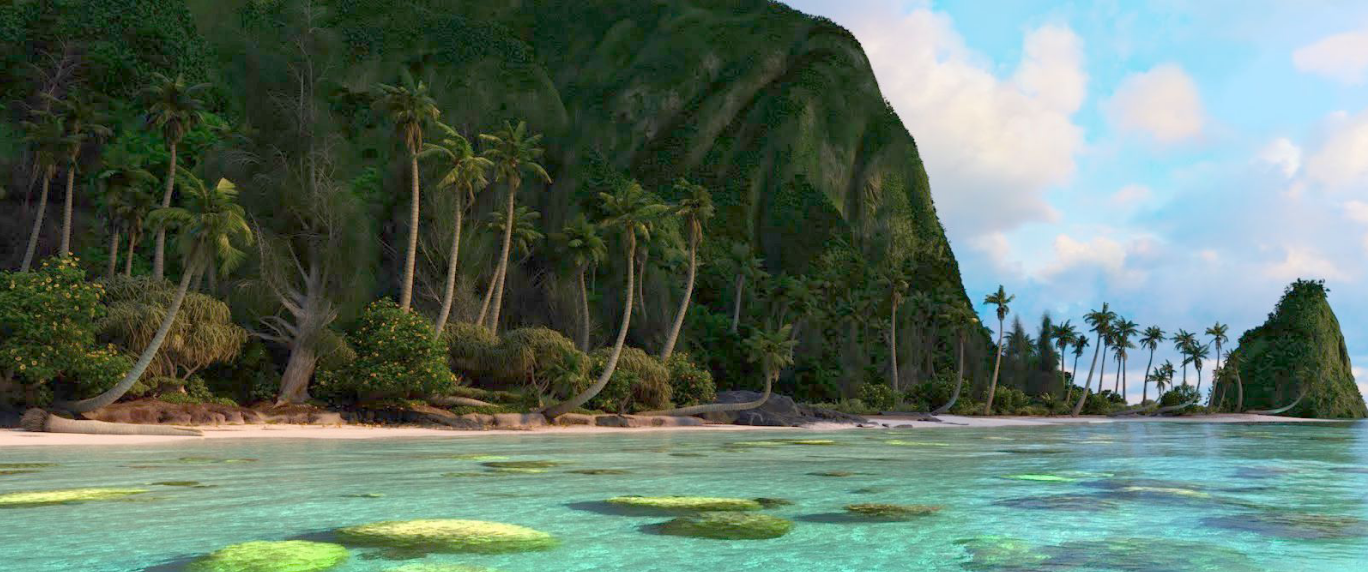
\includegraphics[width=1\linewidth]{img/concl/moana.png}
	\caption{The Moana Island Scene provided by Walt Disney Animation Studios \cite{moana2021}.}
	\label{fig:moana}
\end{figure}

\section{Future work}

\todo{traingle meshes csg'd with bvh}

\begin{figure}[!tbp]
	\centering
	\subfloat{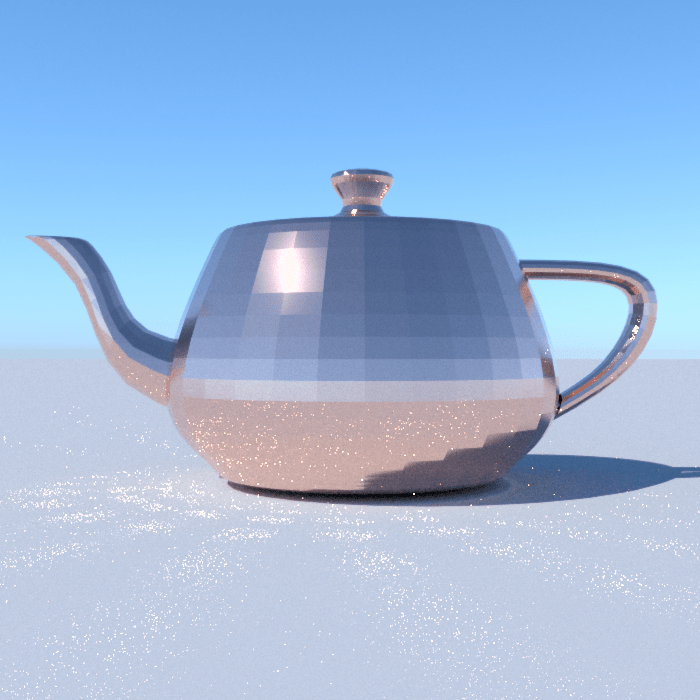
\includegraphics[width=.4\textwidth]{img/concl/teapotEmbree.png}}
	\hfill
	\subfloat{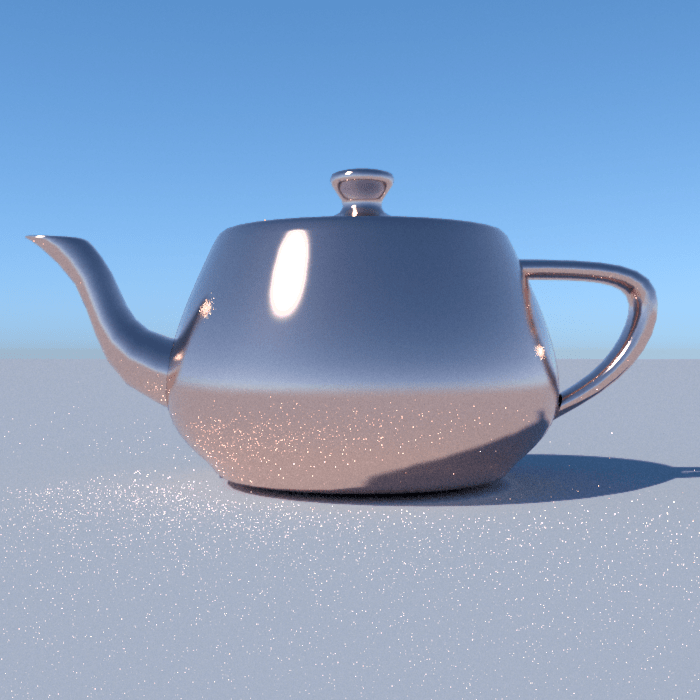
\includegraphics[width=.4\textwidth]{img/concl/teapotNormal.png}}
	\caption{Comparison between the resulting image of a scene containing the Utah teapot by ray tracing with and without Embree support.}
	\label{fig:teapot}
\end{figure}
